\documentclass[12pt,preprint, authoryear]{elsarticle}

\usepackage{lmodern}
%%%% My spacing
\usepackage{setspace}
\setstretch{1.2}
\DeclareMathSizes{12}{14}{10}{10}

% Wrap around which gives all figures included the [H] command, or places it "here". This can be tedious to code in Rmarkdown.
\usepackage{float}
\let\origfigure\figure
\let\endorigfigure\endfigure
\renewenvironment{figure}[1][2] {
    \expandafter\origfigure\expandafter[H]
} {
    \endorigfigure
}

\let\origtable\table
\let\endorigtable\endtable
\renewenvironment{table}[1][2] {
    \expandafter\origtable\expandafter[H]
} {
    \endorigtable
}


\usepackage{ifxetex,ifluatex}
\usepackage{fixltx2e} % provides \textsubscript
\ifnum 0\ifxetex 1\fi\ifluatex 1\fi=0 % if pdftex
  \usepackage[T1]{fontenc}
  \usepackage[utf8]{inputenc}
\else % if luatex or xelatex
  \ifxetex
    \usepackage{mathspec}
    \usepackage{xltxtra,xunicode}
  \else
    \usepackage{fontspec}
  \fi
  \defaultfontfeatures{Mapping=tex-text,Scale=MatchLowercase}
  \newcommand{\euro}{€}
\fi

\usepackage{amssymb, amsmath, amsthm, amsfonts}

\def\bibsection{\section*{References}} %%% Make "References" appear before bibliography


\usepackage[round]{natbib}

\usepackage{longtable}
\usepackage[margin=2.3cm,bottom=2cm,top=2.5cm, includefoot]{geometry}
\usepackage{fancyhdr}
\usepackage[bottom, hang, flushmargin]{footmisc}
\usepackage{graphicx}
\numberwithin{equation}{section}
\numberwithin{figure}{section}
\numberwithin{table}{section}
\setlength{\parindent}{0cm}
\setlength{\parskip}{1.3ex plus 0.5ex minus 0.3ex}
\usepackage{textcomp}
\renewcommand{\headrulewidth}{0.2pt}
\renewcommand{\footrulewidth}{0.3pt}

\usepackage{array}
\newcolumntype{x}[1]{>{\centering\arraybackslash\hspace{0pt}}p{#1}}

%%%%  Remove the "preprint submitted to" part. Don't worry about this either, it just looks better without it:
\makeatletter
\def\ps@pprintTitle{%
  \let\@oddhead\@empty
  \let\@evenhead\@empty
  \let\@oddfoot\@empty
  \let\@evenfoot\@oddfoot
}
\makeatother

 \def\tightlist{} % This allows for subbullets!

\usepackage{hyperref}
\hypersetup{breaklinks=true,
            bookmarks=true,
            colorlinks=true,
            citecolor=blue,
            urlcolor=blue,
            linkcolor=blue,
            pdfborder={0 0 0}}


% The following packages allow huxtable to work:
\usepackage{siunitx}
\usepackage{multirow}
\usepackage{hhline}
\usepackage{calc}
\usepackage{tabularx}
\usepackage{booktabs}
\usepackage{caption}


\newenvironment{columns}[1][]{}{}

\newenvironment{column}[1]{\begin{minipage}{#1}\ignorespaces}{%
\end{minipage}
\ifhmode\unskip\fi
\aftergroup\useignorespacesandallpars}

\def\useignorespacesandallpars#1\ignorespaces\fi{%
#1\fi\ignorespacesandallpars}

\makeatletter
\def\ignorespacesandallpars{%
  \@ifnextchar\par
    {\expandafter\ignorespacesandallpars\@gobble}%
    {}%
}
\makeatother

\newenvironment{CSLReferences}[2]{%
}

\urlstyle{same}  % don't use monospace font for urls
\setlength{\parindent}{0pt}
\setlength{\parskip}{6pt plus 2pt minus 1pt}
\setlength{\emergencystretch}{3em}  % prevent overfull lines
\setcounter{secnumdepth}{5}

%%% Use protect on footnotes to avoid problems with footnotes in titles
\let\rmarkdownfootnote\footnote%
\def\footnote{\protect\rmarkdownfootnote}
\IfFileExists{upquote.sty}{\usepackage{upquote}}{}

%%% Include extra packages specified by user
\usepackage{booktabs}
\usepackage{longtable}
\usepackage{array}
\usepackage{multirow}
\usepackage{wrapfig}
\usepackage{float}
\usepackage{colortbl}
\usepackage{pdflscape}
\usepackage{tabu}
\usepackage{threeparttable}
\usepackage{threeparttablex}
\usepackage[normalem]{ulem}
\usepackage{makecell}
\usepackage{xcolor}

%%% Hard setting column skips for reports - this ensures greater consistency and control over the length settings in the document.
%% page layout
%% paragraphs
\setlength{\baselineskip}{12pt plus 0pt minus 0pt}
\setlength{\parskip}{12pt plus 0pt minus 0pt}
\setlength{\parindent}{0pt plus 0pt minus 0pt}
%% floats
\setlength{\floatsep}{12pt plus 0 pt minus 0pt}
\setlength{\textfloatsep}{20pt plus 0pt minus 0pt}
\setlength{\intextsep}{14pt plus 0pt minus 0pt}
\setlength{\dbltextfloatsep}{20pt plus 0pt minus 0pt}
\setlength{\dblfloatsep}{14pt plus 0pt minus 0pt}
%% maths
\setlength{\abovedisplayskip}{12pt plus 0pt minus 0pt}
\setlength{\belowdisplayskip}{12pt plus 0pt minus 0pt}
%% lists
\setlength{\topsep}{10pt plus 0pt minus 0pt}
\setlength{\partopsep}{3pt plus 0pt minus 0pt}
\setlength{\itemsep}{5pt plus 0pt minus 0pt}
\setlength{\labelsep}{8mm plus 0mm minus 0mm}
\setlength{\parsep}{\the\parskip}
\setlength{\listparindent}{\the\parindent}
%% verbatim
\setlength{\fboxsep}{5pt plus 0pt minus 0pt}



\begin{document}



\begin{frontmatter}  %

\title{Question 1}

% Set to FALSE if wanting to remove title (for submission)




\author[Add1]{Wesley James Williams}
\ead{21691126@sun.ac.za}





\address[Add1]{Stellenbosch University, South Africa}

\cortext[cor]{Corresponding author: Wesley James Williams}

\begin{abstract}
\small{
Answers the Question
}
\end{abstract}

\vspace{1cm}





\vspace{0.5cm}

\end{frontmatter}

\setcounter{footnote}{0}



%________________________
% Header and Footers
%%%%%%%%%%%%%%%%%%%%%%%%%%%%%%%%%
\pagestyle{fancy}
\chead{}
\rhead{}
\lfoot{}
\rfoot{\footnotesize Page \thepage}
\lhead{}
%\rfoot{\footnotesize Page \thepage } % "e.g. Page 2"
\cfoot{}

%\setlength\headheight{30pt}
%%%%%%%%%%%%%%%%%%%%%%%%%%%%%%%%%
%________________________

\headsep 35pt % So that header does not go over title




\hypertarget{porfolio-construction}{%
\section{Porfolio Construction}\label{porfolio-construction}}

I present porfolios constructed with different risk metrics that abide
by the following constraint

\begin{itemize}
\item Long-only strategy;
\itemWhen using covariance and mean forecasts, use a look-back of less than 3 years;
\item Do not hold any assets with less than 3 years’ returns data;
\item Apply Quarterly Rebalancing;
\item Limit exposure to Bonds and credit instruments at 25%;
\item Limit exposure to Equities at 60%;
\item Limit single asset exposure at 40%;
\item Data after 2010.
\end{itemize}

\begin{tabular}{l|r|r|r|r|l|r}
\hline
Tickers & mv & minvol & erc & riskeff & date & Look\_Back\_Period\\
\hline
ADXY Index & 0.0769231 & 0.2500000 & 0.1102687 & 0.0769231 & 2011-04-29 & 36\\
\hline
BCOMTR Index & 0.0769231 & 0.0530710 & 0.0454807 & 0.0769231 & 2011-04-29 & 36\\
\hline
DXY Index & 0.0769231 & 0.2499308 & 0.0100000 & 0.0769231 & 2011-04-29 & 36\\
\hline
LEATTREU Index & 0.0769231 & 0.0100000 & 0.1079268 & 0.0769231 & 2011-04-29 & 36\\
\hline
LGAGTRUH Index & 0.0769231 & 0.1214055 & 0.1794023 & 0.0769231 & 2011-04-29 & 36\\
\hline
LGCPTRUH Index & 0.0769231 & 0.0100000 & 0.0681874 & 0.0769231 & 2011-04-29 & 36\\
\hline
LP05TREH Index & 0.0769231 & 0.0100000 & 0.0775276 & 0.0769231 & 2011-04-29 & 36\\
\hline
LUACTRUU Index & 0.0769231 & 0.0100000 & 0.0594818 & 0.0769231 & 2011-04-29 & 36\\
\hline
LUAGTRUU Index & 0.0769231 & 0.2455928 & 0.2209793 & 0.0769231 & 2011-04-29 & 36\\
\hline
MSCI\_ACWI & 0.0769231 & 0.0100000 & 0.0281465 & 0.0769231 & 2011-04-29 & 36\\
\hline
MSCI\_Jap & 0.0769231 & 0.0100000 & 0.0398264 & 0.0769231 & 2011-04-29 & 36\\
\hline
MSCI\_RE & 0.0769231 & 0.0100000 & 0.0214806 & 0.0769231 & 2011-04-29 & 36\\
\hline
MSCI\_USA & 0.0769231 & 0.0100000 & 0.0312919 & 0.0769231 & 2011-04-29 & 36\\
\hline
\end{tabular}

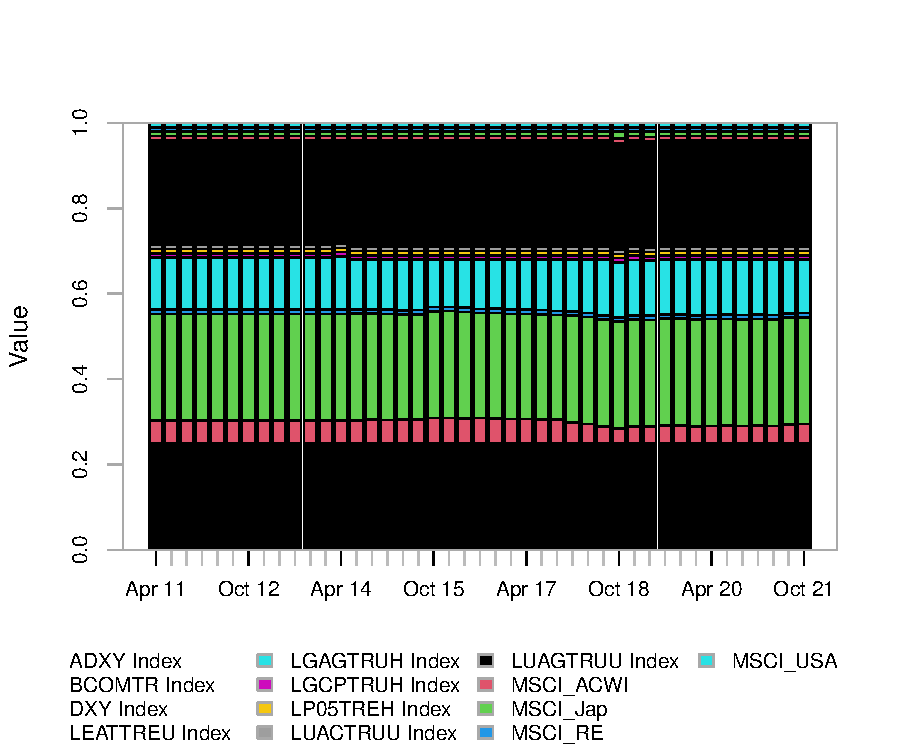
\includegraphics{Question-6_files/figure-latex/unnamed-chunk-4-1.pdf}

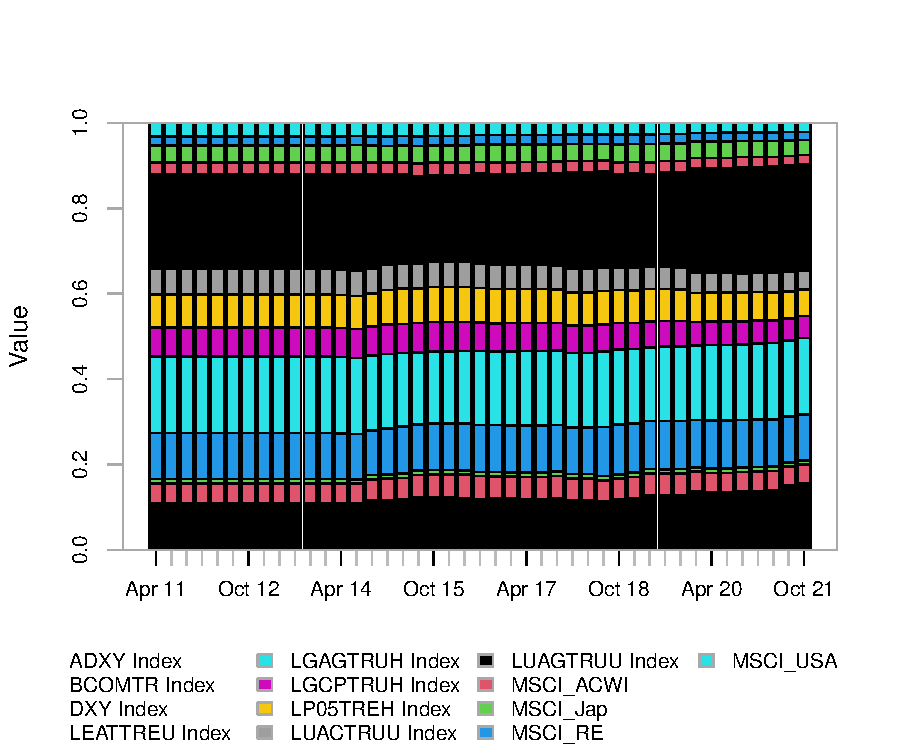
\includegraphics{Question-6_files/figure-latex/unnamed-chunk-5-1.pdf}

\begin{tabular}{l|r|r|r|r|l|r}
\hline
Tickers & mv & minvol & erc & riskeff & date & Look\_Back\_Period\\
\hline
ADXY Index & 0.0769231 & 0.2500000 & 0.1102687 & 0.0769231 & 2011-04-29 & 24\\
\hline
BCOMTR Index & 0.0769231 & 0.0530710 & 0.0454807 & 0.0769231 & 2011-04-29 & 24\\
\hline
DXY Index & 0.0769231 & 0.2499308 & 0.0100000 & 0.0769231 & 2011-04-29 & 24\\
\hline
LEATTREU Index & 0.0769231 & 0.0100000 & 0.1079268 & 0.0769231 & 2011-04-29 & 24\\
\hline
LGAGTRUH Index & 0.0769231 & 0.1214055 & 0.1794023 & 0.0769231 & 2011-04-29 & 24\\
\hline
LGCPTRUH Index & 0.0769231 & 0.0100000 & 0.0681874 & 0.0769231 & 2011-04-29 & 24\\
\hline
LP05TREH Index & 0.0769231 & 0.0100000 & 0.0775276 & 0.0769231 & 2011-04-29 & 24\\
\hline
LUACTRUU Index & 0.0769231 & 0.0100000 & 0.0594818 & 0.0769231 & 2011-04-29 & 24\\
\hline
LUAGTRUU Index & 0.0769231 & 0.2455928 & 0.2209793 & 0.0769231 & 2011-04-29 & 24\\
\hline
MSCI\_ACWI & 0.0769231 & 0.0100000 & 0.0281465 & 0.0769231 & 2011-04-29 & 24\\
\hline
MSCI\_Jap & 0.0769231 & 0.0100000 & 0.0398264 & 0.0769231 & 2011-04-29 & 24\\
\hline
MSCI\_RE & 0.0769231 & 0.0100000 & 0.0214806 & 0.0769231 & 2011-04-29 & 24\\
\hline
MSCI\_USA & 0.0769231 & 0.0100000 & 0.0312919 & 0.0769231 & 2011-04-29 & 24\\
\hline
\end{tabular}

\begin{tabular}{l|r|r|r|r|l|r}
\hline
Tickers & mv & minvol & erc & riskeff & date & Look\_Back\_Period\\
\hline
ADXY Index & 0.0769231 & 0.2500000 & 0.1102687 & 0.0769231 & 2011-04-29 & 12\\
\hline
BCOMTR Index & 0.0769231 & 0.0530710 & 0.0454807 & 0.0769231 & 2011-04-29 & 12\\
\hline
DXY Index & 0.0769231 & 0.2499308 & 0.0100000 & 0.0769231 & 2011-04-29 & 12\\
\hline
LEATTREU Index & 0.0769231 & 0.0100000 & 0.1079268 & 0.0769231 & 2011-04-29 & 12\\
\hline
LGAGTRUH Index & 0.0769231 & 0.1214055 & 0.1794023 & 0.0769231 & 2011-04-29 & 12\\
\hline
LGCPTRUH Index & 0.0769231 & 0.0100000 & 0.0681874 & 0.0769231 & 2011-04-29 & 12\\
\hline
LP05TREH Index & 0.0769231 & 0.0100000 & 0.0775276 & 0.0769231 & 2011-04-29 & 12\\
\hline
LUACTRUU Index & 0.0769231 & 0.0100000 & 0.0594818 & 0.0769231 & 2011-04-29 & 12\\
\hline
LUAGTRUU Index & 0.0769231 & 0.2455928 & 0.2209793 & 0.0769231 & 2011-04-29 & 12\\
\hline
MSCI\_ACWI & 0.0769231 & 0.0100000 & 0.0281465 & 0.0769231 & 2011-04-29 & 12\\
\hline
MSCI\_Jap & 0.0769231 & 0.0100000 & 0.0398264 & 0.0769231 & 2011-04-29 & 12\\
\hline
MSCI\_RE & 0.0769231 & 0.0100000 & 0.0214806 & 0.0769231 & 2011-04-29 & 12\\
\hline
MSCI\_USA & 0.0769231 & 0.0100000 & 0.0312919 & 0.0769231 & 2011-04-29 & 12\\
\hline
\end{tabular}

\newpage

\hypertarget{references}{%
\section*{References}\label{references}}
\addcontentsline{toc}{section}{References}

\hypertarget{refs}{}
\begin{CSLReferences}{0}{0}
\end{CSLReferences}

\bibliography{Tex/ref}





\end{document}
